\documentclass{article}


% Title Page
\title{\Huge \textbf{Simulazioni \textit{n}-body su GPU: approccio naive e Barnes-Hut}}
\author{Relazione del progetto di GPGPU - Damiano Trovato}
\date{}
\usepackage{biblatex}
\addbibresource{report.bib}
\usepackage{booktabs}
\usepackage{longtable}
\usepackage{graphicx} % Per le immagini
\usepackage{amsmath} % Simboli matematici
\usepackage[hidelinks]{hyperref} % Collegamenti ipertestuali
\usepackage{amssymb} % Simboli matematici 2
\usepackage{tikz}
\usepackage{fancyvrb}
\usepackage{multicol}
\usepackage{geometry}
\usepackage{array}
\usepackage{tabularx} % nel preambolo
\usepackage{listings}
\usepackage{algorithm}
\makeatletter
\renewcommand{\ALG@name}{Pseudo-codice}
\makeatother
\usepackage{algpseudocode}
\newcommand{\Break}{\State \textbf{break}}
\newcommand{\Continue}{\State \textbf{continue}}

\renewcommand{\thelstnumber}{\arabic{lstnumber}:}
\lstdefinestyle{mystyle}{          
	numbers=left,                    
	numbersep=5pt             
}
\lstset{style=mystyle}

\makeatother
\geometry{
	a4paper,
	total={160mm,260mm},
	left=20mm,
	top=18mm,
}
% RIDENOMINAZIONI
\renewcommand{\contentsname}{Indice}
\renewcommand{\figurename}{\textbf{Immagine}}


\begin{document}

	\maketitle
	
\begin{abstract}
Con la seguente relazione si documenta la realizzazione di codici per simulazioni $n$-body tramite soluzioni parallele su GPU. Si trattano quindi aspetti degni di nota, quali gli algoritmi, i metodi numerici,  le ottimizzazioni e delle analisi relative alle performance.  Le soluzioni presentate saranno le seguenti: un'approccio naive su GPU, un approccio approssimato Barnes-Hut totalmente su GPU (con quad-tree seriale), un approccio approssimato Barnes-Hut ibrido GPU-CPU, e una variazione sul secondo algoritmo, implementando la riduzione tramite sliding window (con memoria locale).
\end{abstract}
\newpage
\tableofcontents
\newpage

\section{Introduzione}
In questa sezione offriamo un'introduzione al progetto, dando una definizione del problema $n$-body, i dettagli fisici e matematici e come verranno sviluppati i test.

\subsection{Simulazioni \textit{n}-body}
Una simulazione a $n$ corpi permette di calcolare l'evoluzione temporale di un sistema costituito da, appunto, $n$ corpi che interagiscono tra loro con delle forze che dipendono dalla simulazione. Queste simulazioni sono fondamentali, in quanto ogni problema a $n$ corpi non banale, e con configurazione non banale\footnote{assenza totale di forze, o configurazioni con determinate simmetrie.}, non dispone di una soluzione analitica.

\begin{figure}[htbp]
	\centering
	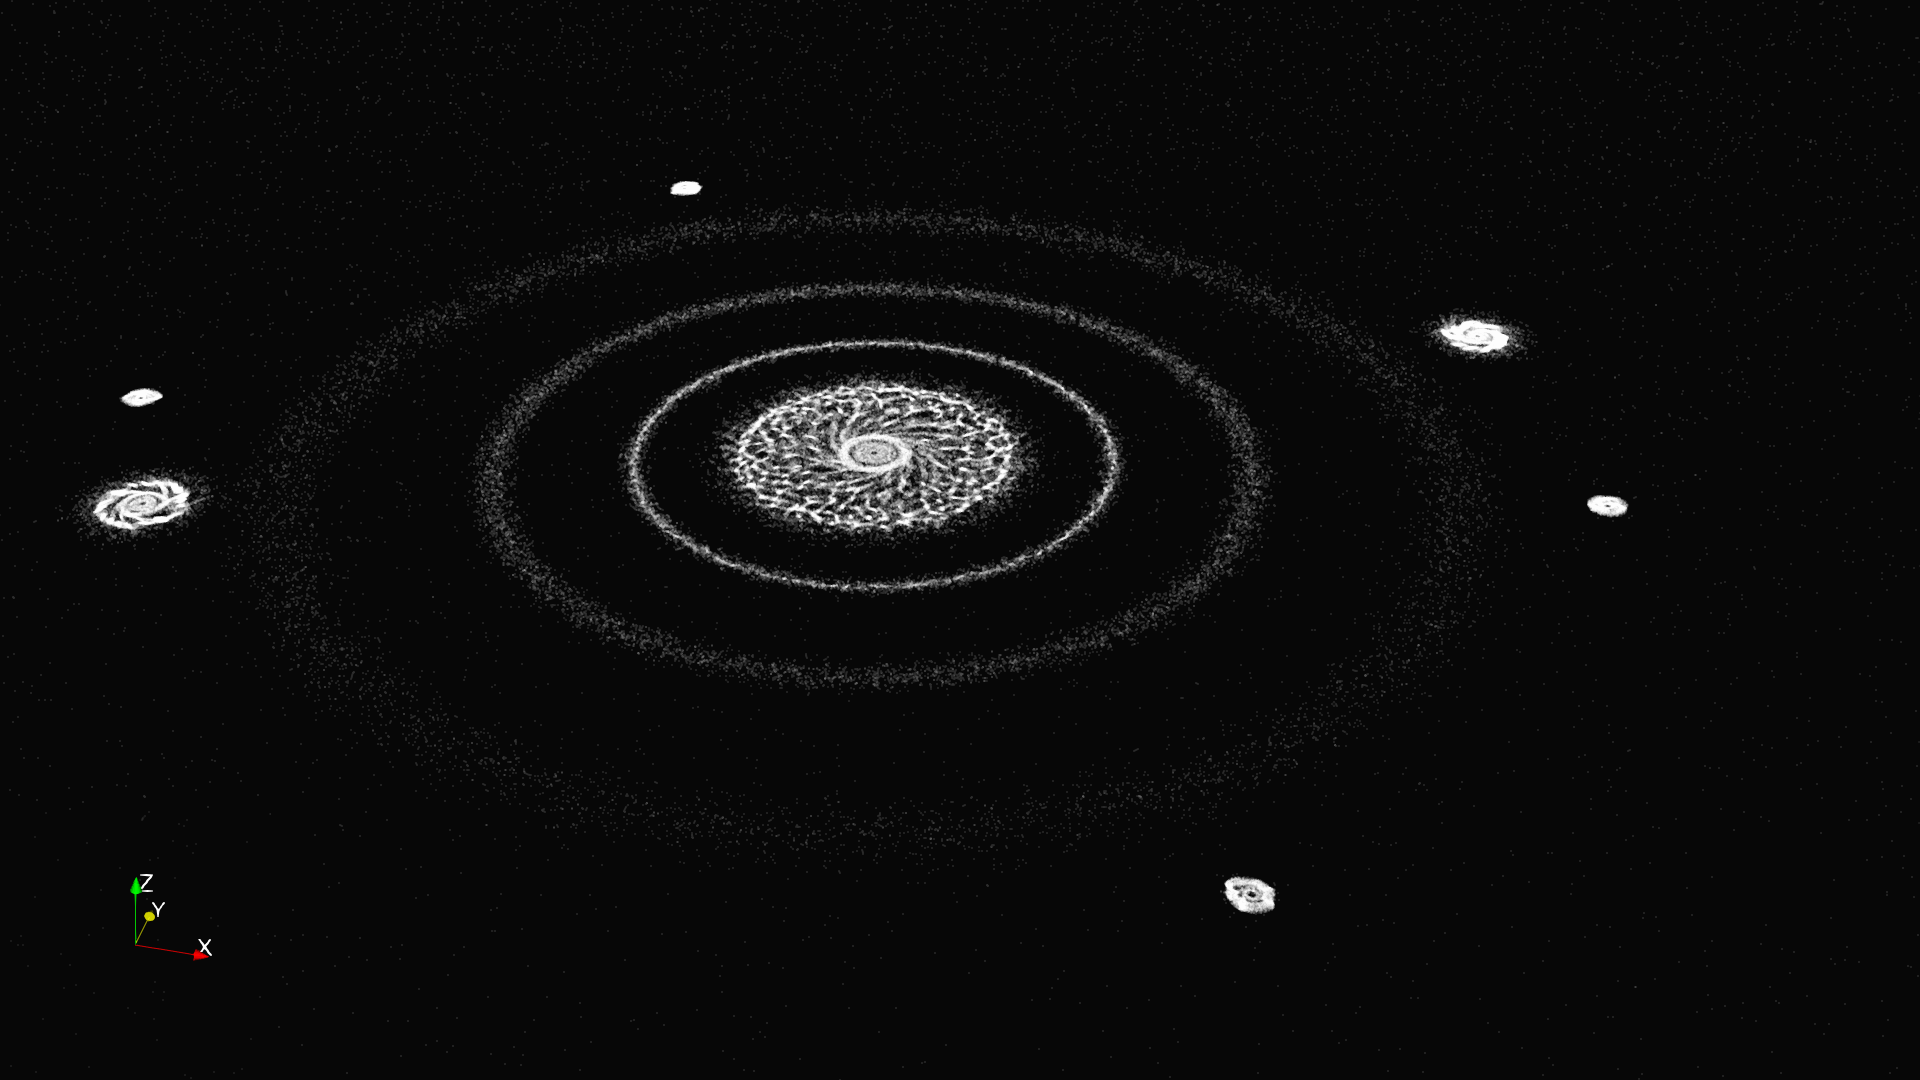
\includegraphics[width=0.8\linewidth]{../images/GALASSIA3}
	\caption{Una demo a 180k corpi: \url{https://youtu.be/oSdXonzxpXk?si=4AL8uCfM6irIlBcW}}
\end{figure}
%
Sono fondamentali nell'ambito dell'astrofisica computazionale, offrendo ad esempio soluzioni per osservare l'evoluzione di sistemi cosmologici.

\newpage
	\subsection{Aspetti fisici e matematici}
	Si offre una lista delle formule matematiche che rendono fattibili le simulazioni realizzate all'interno del progetto. Le seguenti formule sono state prese dal video~\cite{deadlock2023nbody}.
	
	\paragraph{Legge di gravitazione universale} La seguente formula detta l'attrazione che agisce tra due corpi rispettivamente di massa $m_1$ ed $m_2$, situate a distanza $|r|$. Questa grandezza è direttamente proporzionale al prodotto delle masse e inversamente proporzionale al quadrato della distanza, ossia:
	\begin{equation}
	F = G \frac{m_1m_2}{|r|^2} \hat r = G \frac{m_1m_2}{|r|^2} \cdot \frac{r}{|r|} = G \frac{m_1m_2}{|r|^3} r.
	\end{equation}
	%
	In natura $G$ è una costante minuscola che rende l'attrazione tra i corpi rilevante solo se i corpi hanno massa elevatissima o distanza reciproca ridotta. Ai fini della simulazione, questa costante verrà impostata a $G=0.2$. $\hat r$ indica invece il versore\footnote{vettore unitario} che punta da $m_1$ a $m_2$, ottenuto normalizzando $r$. Sostituiamo quindi $\hat r$ con la sua formula esplicita.
	\paragraph{Dalla forza all'accelerazione}
	Supponiamo sul corpo $m_1$ agisca una determinata forza $F$:
	\begin{equation}
	F = m_1 a \Rightarrow a = \frac{F}{m_1} = G \frac{m_2}{|r|^3} r.
	\end{equation}
	%
	In definitiva, l'accelerazione che agisce su un corpo $m_i$ è data da:
	\begin{equation}
	a_i = \sum_{j=0,\, j \neq i}^{n-1} G \frac{m_j}{|r_j|^3} r_j.
	\end{equation}
	\paragraph{Dall'accelerazione alla velocità} L'accelerazione è la derivata della velocità sul tempo, possiamo quindi calcolare la velocità di un corpo tramite
	
	\begin{equation}
	a = \frac{dv}{dt} \Rightarrow adt = dv,
	\end{equation}
	%
	fissando un valore di $dt = \verb*|delta_time|$.
	
	\paragraph{Dalla velocità allo spostamento}
	\begin{equation}
	x = x_0 + v dt
	\end{equation}
	%
	dove $dt = \verb*|delta_time|$.
	
	\subsection{Metodo numerico di integrazione: leapfrog}
	\begin{figure}[tbph]
		\centering
		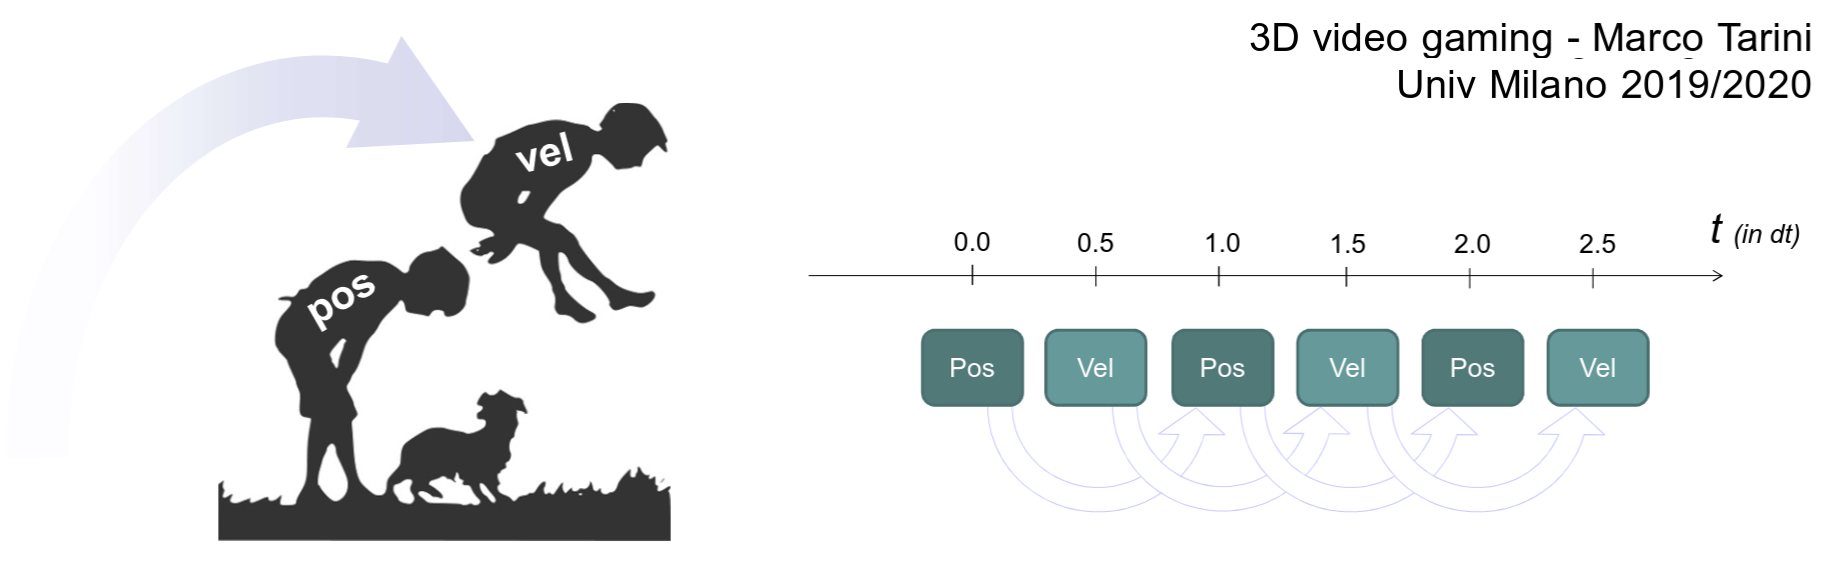
\includegraphics[width=1\linewidth]{../images/leapfrog}
		\label{fig:leapfrog}
	\end{figure}
	%
	Il metodo numerico utilizzato nella simulazione, è noto come metodo leapfrog, o metodo della cavallina. Il nome deriva dal modo in cui si alterna l'integrazione della velocità a quella del tempo.
	
	
	\begin{algorithm}[htp]
		\caption{Integrazione Leapfrog}
		\begin{algorithmic}[1]
		\State Calcola l'accelerazione
		\State Aggiorna la velocità per $dt/2$
		\For{Numero di iterazioni}
			\State Aggiorna la posizione per $dt$
			\State Calcola l'accelerazione
			\State Aggiorna la velocità per $dt$
		\EndFor
		\end{algorithmic}
	\end{algorithm}
	
	Questo metodo numerico, sfasando di $dt/2$ l'integrazione della velocità e della posizione, ottiene errore ridotto, miglior comportamento asintotico e conservazione dell'energia del sistema, rispetto al metodo di Eulero. Sono tecniche di integrazione egualmente onerose, ma il metodo Leapfrog è più accurato e totalmente reversibile~\cite{tarini2019gamephysics3}.
	
	\subsection{Studio delle performance su hardware}
	L'hardware a disposizione per i test, è il seguente:
	\begin{itemize}
		\item \textbf{AMD Radeon RX 6600 CLD 8GB} (discreta);
		\item \textbf{Intel Core Ultra 9 285H - Intel Arc Pro 130T/140T} (integrata);
		\item \textbf{AMD Ryzen 7 7700 - gfx1036} (integrata), ma questa verrà usata solo sull'algoritmo naive, perché le prestazioni sull'algoritmo Barnes-Hut sono disastrose e poco interessanti da studiare.
	\end{itemize}
	%
	In tutte le soluzioni affrontate, verranno omesse le operazioni di scrittura a disco dei frame della simulazione, che rappresentano una grande fonte di overhead, ma che sono anche fuori dallo scope del progetto.
	
	Le nostre valutazioni avverranno rispetto ad un numero crescente di corpi $n$ da 10 a $\sim 180 000$. Per ogni simulazione, valutiamo il calcolo di 10 frame, in modo da ridurre l'effetto della varianza sul singolo tempo di esecuzione del kernel, su un frame particolarmente fortunato (o sfortunato).
	\newpage
	
	\section{Simulazione parallela naive su GPU}
	Il primo approccio alla simulazione di sistemi a $n$ corpi che si è deciso di realizzare, è una soluzione parallela basata sull'algoritmo naive, con complessità computazionale $\mathcal{O}(n^2)$. Consiste banalmente nel calcolo brute-force di tutte le interazioni corpo-a-corpo.
	
	
	\subsection{Kernel fondamentali e ottimizzazioni}
	
	\paragraph{Calcolo dell'accelerazione naive}
	Il primo kernel che trattiamo, viene eseguito su ogni corpo per ogni istante della simulazione, e permette il calcolo dell'accelerazione su ogni corpo.
	\begin{algorithm}
		\caption{Kernel per il calcolo dell'accelerazione di un corpo}
		\begin{algorithmic}[1]
			\Require array dei corpi $C$, $n = |C|$
			\State $i \gets$ id globale del work-item
			\If{$i >= n$}
			\Return
			\Comment Usciamo dal programma se il work-item è fuori dal dominio dell'input
			\EndIf
			\State $a \gets 0$
			\ForAll{$j \in \{0,\, \dots, n-1\}$}
			\If{$i = j$} \Continue 
			\EndIf
			\State $ r \gets C_{pos}[i] - C_{pos}[j]$
			\State $r = \max(r,\, \varepsilon)$
			\State $a \gets G \frac{C_{mass}[j]}{|r|^3} r + a $
			\EndFor
			\State $C_{acc}[i] \gets a$
		\end{algorithmic}
	\end{algorithm}
	%
	dalla teoria all'implementazione, subentrano delle ottimizzazioni. Il calcolo di $\dfrac{1}{|r^3|}$ è infatti ottimizzato col calcolo della radice quadrata inversa su $r$ al cubo (notoriamente più veloce del calcolo esplicito della radice quadrata e della divisione).
	
	\begin{figure}[tph]
		\centering
		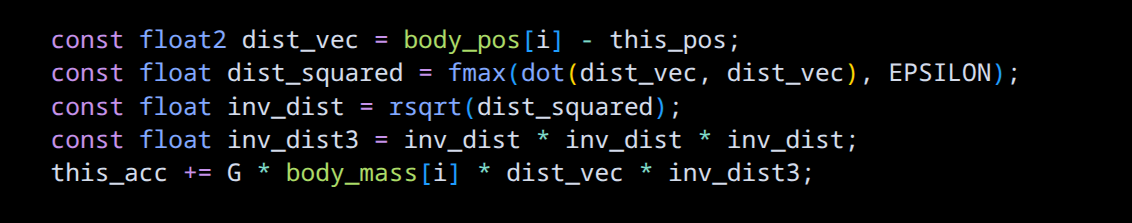
\includegraphics[width=1\linewidth]{../images/compute-accel-naive}
	\end{figure}
	%
	Osserviamo inoltre una funzione $\max(r,\, \varepsilon)$, con $\varepsilon$ valore arbitrariamente piccolo per evitare che $|r|^3 \to 0$ (con conseguente accelerazione $\to \pm\infty$) o peggio ancora $|r|^3 = 0$, che causerebbe un errore di divisione per zero. Questo problema si pone perché nella simulazione non consideriamo collisioni, i corpi possono passarsi attraverso, ottenendo valori molto piccoli di $r$. Scegliamo il valore $\varepsilon$ sperimentalmente.
	
	\paragraph{Calcolo della velocità}
	Il seguente kernel è invece dedicato al calcolo della velocità dall'accelerazione. Il delta tempo $dt$ è un argomento, in quanto necessario per il metodo leapfrog.
	\begin{algorithm}[htbp]
		\caption{Kernel per il calcolo della velocità}
		\begin{algorithmic}[1]
			\Require array dei corpi $C$, $n = |C|$, delta tempo $dt$
			\State $i \gets$ id globale del work-item
			\If{$i >= n$}
			\Return
			\Comment Usciamo dal programma se il work-item è fuori dal dominio dell'input
			\EndIf
			\State $C_{vel}[i] \gets C_{vel}[i] + C_{acc}[i] \cdot dt$
		\end{algorithmic}
	\end{algorithm}
	
	\paragraph{Calcolo della posizione}
	L'ultimo kernel della simulazione naive è dedicato all'aggiornamento della posizione. 
	\begin{algorithm}[htbp]
		\caption{Kernel per il calcolo della posizione}
		\begin{algorithmic}[1]
			\Require array dei corpi $C$, $n = |C|$, delta tempo $dt$
			\State $i \gets$ id globale del work-item
			\If{$i >= n$}
			\Return
			\Comment Usciamo dal programma se il work-item è fuori dal dominio dell'input
			\EndIf
			\State $C_{pos}[i] \gets C_{pos}[i] + C_{vel}[i] \cdot dt$
		\end{algorithmic}
	\end{algorithm}
	
	\newpage
	\subsection{Codice host}
	
		\begin{algorithm}[htp]
		\caption{Simulazione $n$-body naive}
		\begin{algorithmic}[1]
		\Require array dei corpi $C$, $n = |C|$, delta tempo $dt$, numero di  iterazioni $t$
		\State lancia $n$ kernel \textbf{accelerazione naive} su $C$ con delta tempo $dt$ 
		\State lancia $n$ kernel \textbf{calcolo velocità} su $C$ con delta tempo $dt/2$ 
		\For{t}
		\State lancia $n$ kernel \textbf{calcolo posizione} su $C$ con delta tempo $dt$ 
		\State lancia $n$ kernel \textbf{accelerazione naive} su $C$ con delta tempo $dt$ 
		\State lancia $n$ kernel \textbf{calcolo velocità} su $C$ con delta tempo $dt$ 
		\EndFor
		
		\end{algorithmic}
	\end{algorithm}
	%
	In realtà, per ogni kernel lanciato, il numero di kernel è quasi sempre arrotondato al primo multiplo di 32 più grande di $n$, per evitare che le performance vengano penalizzate (aggiungerei, in maniera disastrosa) da un numero primo di particelle.
	
	\subsection{Numero di accessi in memoria globale}
	Per avere una prospettiva più consapevole nello studio delle prestazioni dell'algoritmo, andiamo a osservare il numero di accessi in memoria globale, che sappiamo rappresentare una delle più grandi fonti di bottleneck nell'esecuzione dei kernel degli programmi su GPU. Considerando un solo kernel, questo effettua il seguente numero di accessi in memoria globale:
	
	\begin{itemize}
		\item \textbf{aggiornamento posizione},  uno alla velocità e uno alla posizione, $\mathcal O(1)$;
		\item \textbf{aggiornamento velocità}, uno all'accelerazione e uno alla velocità, $\mathcal O(1)$;
		\item \textbf{aggiornamento accelerazione}, $n$ alle posizioni, $n$ alle masse, 1 all'accelerazione, $\mathcal O(n)$;
	\end{itemize}
	con $n$ numero di corpi.
	
	\subsection{Benchmarking}
	Valutiamo finalmente le prestazioni dell'algoritmo. Dai grafici delle successive pagine, emergono un paio di osservazioni: entrambe le GPU integrate performano in maniera simile sul calcolo di posizione e velocità. In generale, il calcolo di posizione e velocità sembra crescere linearmente in funzione del numero di corpi.  
	
\begin{figure}[tbph]
	\centering
	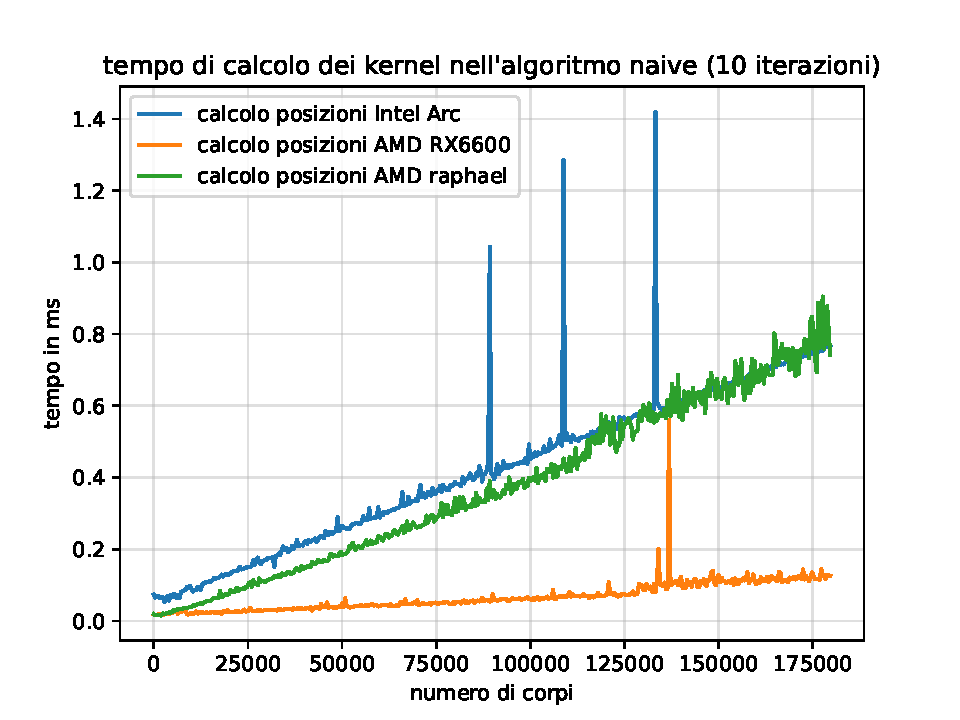
\includegraphics[width=0.85\linewidth]{../images/naive_position_manygpu}
	\label{fig:naivepositionmanygpu}
	\caption{Tempo di calcolo della posizione, in funzione del numero di corpi, valutato su tre schede video differenti. In arancione, abbiamo l'unica GPU discreta, la RX6600 di casa AMD.}
\end{figure}

\begin{figure}[tbph]
	\centering
	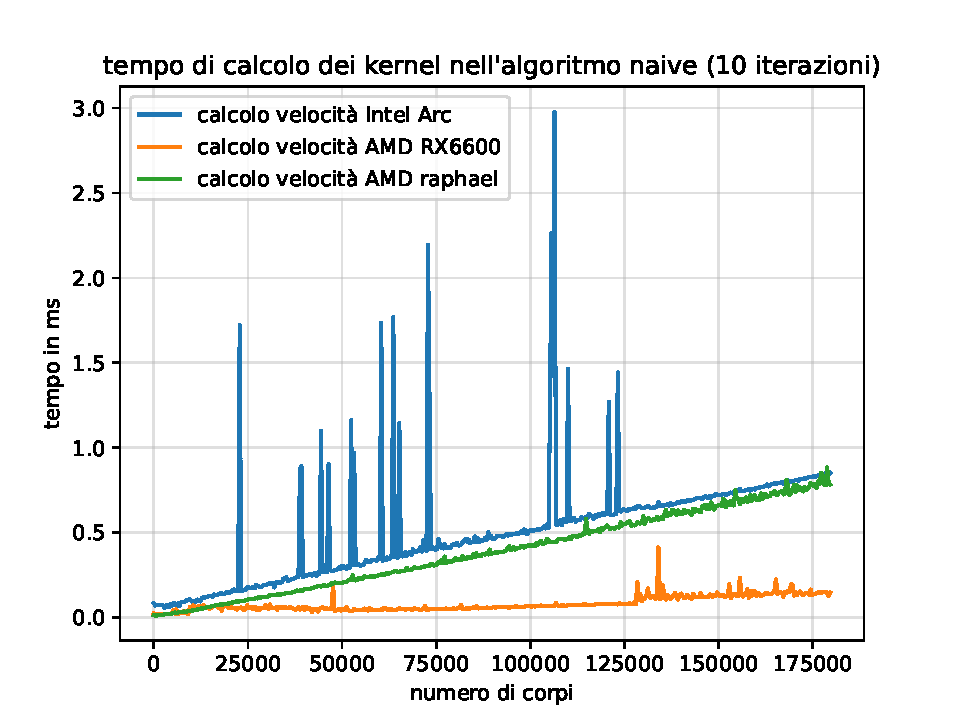
\includegraphics[width=0.85\linewidth]{../images/naive_speed_manygpu}
	\caption{Tempo di calcolo della velocità, in funzione del numero di corpi.}
	\label{fig:naivespeedmanygpu}
\end{figure}

\newpage
Meno fortunato è il calcolo dell'accelerazione dei corpi. L'alto numero di operazioni e di accessi alla memoria globale, demolisce totalmente le performance della grafica integrata del Ryzen 7 7700 (Raphael), meno avanzata se messa a confronto con le performance della grafica integrata Intel.

\begin{figure}[tbph]
	\centering
	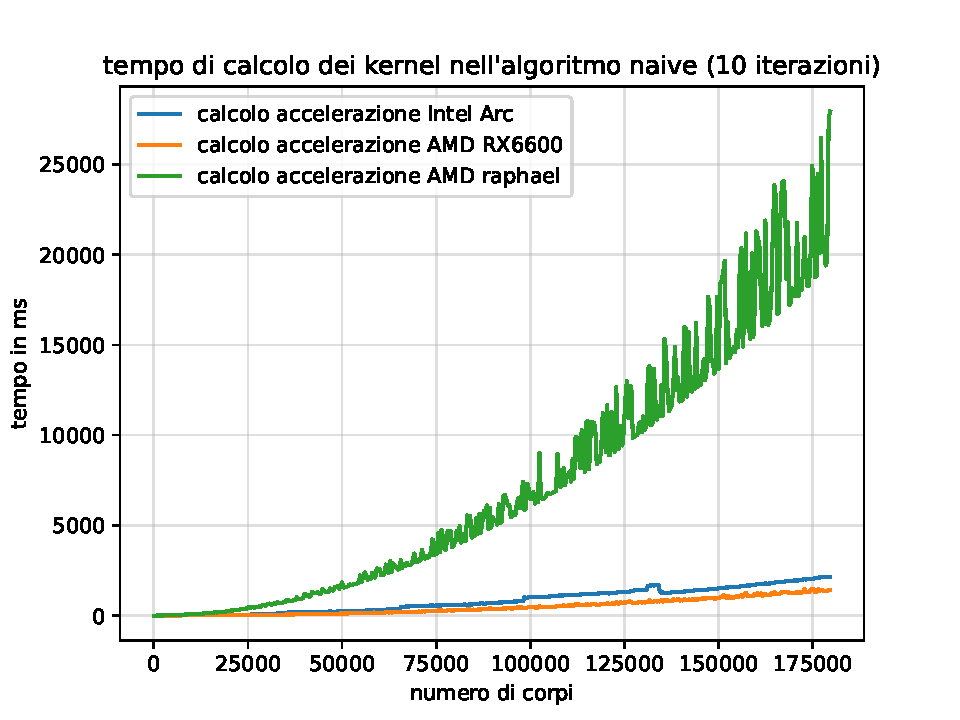
\includegraphics[width=0.73\linewidth]{../images/naive_acc_manygpu}
	\caption{Tempo di calcolo dell'accelerazione, in funzione del numero di corpi.}
	\label{fig:naiveaccmanygpu}
\end{figure}
\begin{figure}[tbph]
	\centering
	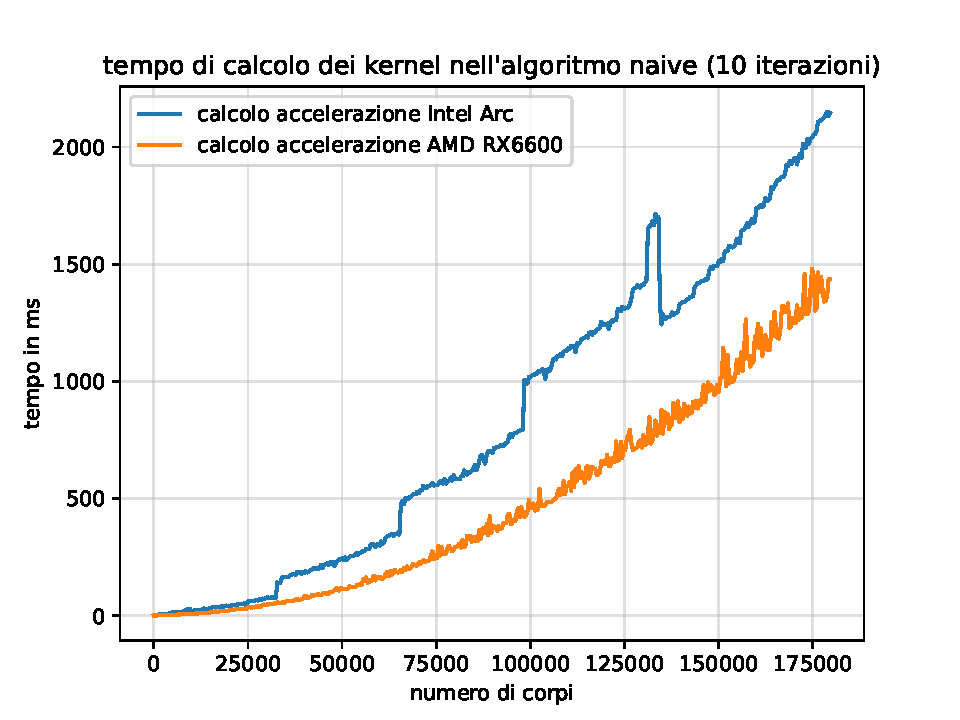
\includegraphics[width=0.72\linewidth]{../images/naive_acc_manygpu_no_raphael}
	\label{fig:naiveaccmanygpunoraphael}
	\caption{Ai fini di visualizazione, proponiamo lo stesso grafico precedente escludendo l'AMD Raphael.}
\end{figure}

Seppur tutte le visualizzazioni dei sistemi siano state effettuate in un secondo momento all'interno del software ParaView, è possibile calcolare il tempo massimo ammesso per il calcolo di un fotogramma della simulazione, in contesto realtime. La formula è
\begin{equation}
t = \dfrac{1000}{\text{frame per secondo}}\ \operatorname{ms},
\end{equation}
%
per cui, i tempi per calcolare un frame a 30 FPS dovranno essere al più $t_{30} = 33,33 \operatorname{ms}$, per 60 FPS al più la metà, ossia $t_{60} = 16,6 \operatorname{ms}$. Moltiplichiamo queste quantità per 10, per poter riutilizzare i dati già elaborati.

\begin{figure}[tph]
	\centering
	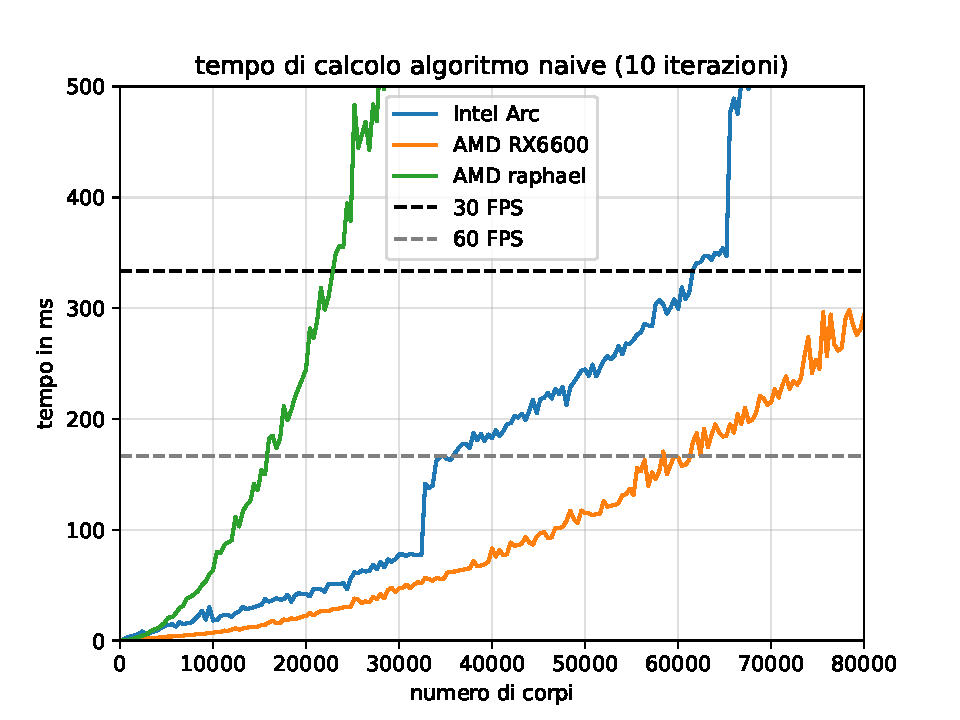
\includegraphics[width=0.85\linewidth]{../images/naive_total_ms}
	\caption{Somma dei tempi dei kernel }
	\label{fig:naivetotalms}
\end{figure}

A 30 FPS, Raphael AMD può simulare 22800 corpi, l'Intel ARC fino a 61200 corpi e l'AMD RX6600 fino a 82800 corpi.
A 60 FPS, Raphael non supera i 15610 corpi, l'Intel ARC i 34400 corpi e l'AMD RX6600 i 58000 corpi. La crescita quadratica dell'algoritmo naive (sia in termini di algoritmo, che in termini di accessi alla memoria globale) è il punto debole dell'algoritmo.

\newpage
	
\section{Simulazione Barnes-Hut totalemente su GPU con costruzione seriale del quadtree}
L'algoritmo Barnes-Hut permette di simulare sistemi a $n$ corpi in maniera approssimata, con precisione arbitraria e complessità asintotica $\mathcal O (n \log n)$. Sfrutta una particolare struttura dati, ossia un quad-tree (figura~\ref{fig:quadtree}), un albero in cui ogni nodo ha quattro figli, per suddividere ricorsivamente lo spazio,  memorizzare valori relativi al sistema e velocizzare il passaggio più oneroso della simulazione brute-force: il calcolo delle forze (o dell'accelerazione), notoriamente un passaggio a complessità $\mathcal O (n^2)$.
%
\begin{figure}[tbph]
	\centering
	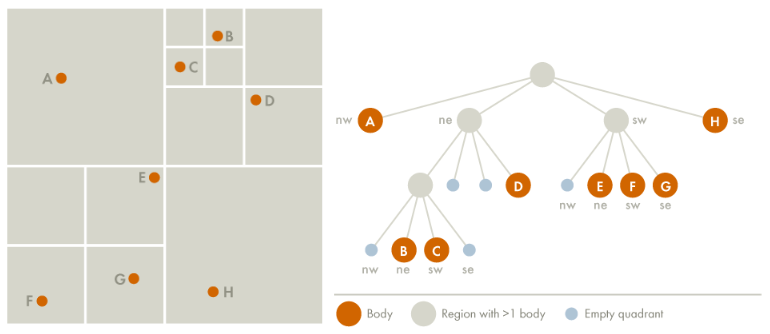
\includegraphics[width=0.75\linewidth]{../images/quadtree}
	\label{fig:quadtree}
	\caption{Bounding box e quad-tree nell'algoritmo Barnes-Hut, immagine tratta da \url{https://arborjs.org/docs/barnes-hut}}
\end{figure}
%
L'idea è la seguente: costruiamo un albero che descrive l'intero sistema, e invece di calcolare l'attrazione tra un corpo $c$ e il resto dei corpi $C$ interrogandoli uno ad uno, si visita l'albero, e per ogni altro nodo ci chiediamo ``posso approssimare tutti i figli di questo nodo ad un unico corpo?''. Lo sviluppo in moltipoli ci dice che questa approssimazione è affidabile quando l'area che include questi corpi non è molto grande e quando la distanza da $c$ è elevata: useremo un parametro $\theta$ soglia, che verrà confrontato proprio al rapporto tra le grandezze appena citate. Quando il criterio è rispettato, si accetta il nodo come approssimazione di tutti i corpi della regione associata, con posizione uguale al centro di massa, e massa uguale alla somma delle masse, altrimenti si continua la visita nell'albero. Su sistemi con molteplici regioni dense, ma molto distanti tra loro, l'algoritmo Barnes-Hut performa estremamente bene. 

Tuttavia l'algoritmo paga l'overhead della costruzione del quad-tree, che richiede non pochi passaggi:
\begin{enumerate}
	\item definizione dell'area dell'intero sistema particellare, ossia la bounding-box;
	\item inserimento di ciascun corpo all'interno dell'albero;
	\item propagazione nei nodi interni delle masse e dei centri di massa dei rispettivi figli.
\end{enumerate}
%
Questi passaggi sono i più costosi dell'algoritmo, ma sono anche alla base del suo vantaggio asintotico.

\newpage
	\subsection{I kernel fondamentali}
	
	\paragraph{Calcolo dei margini della bounding-box}
	I primi kernel sono quelli dedicati alla definizione della dimensione della bounding-box (ossia della radice del quad-tree). Usiamo due riduzione parallele, una per trovare il minimo e l'altra per il massimo dell'intero sistema particellare, sia su $x$ che su $y$. In questo modo, sarà possibile costruire un quadrato (la bounding-box) che conterrà l'intero sistema.
	
	\begin{algorithm}
		\caption{Kernel per la riduzione parallela (ricerca del minimo o massimo)}
		\begin{algorithmic}[1]
			\Require array $A$, array $B$, dimensione dell'input $n$, array $BoundingBox$, flag per l'ultima riduzione
			\State $j \gets$ id globale del work-item
			\State $i \gets 2j$ 
			\If{$i > n$}
				\Return
				\Comment Usciamo dal programma se il work-item è fuori dal dominio dell'input
			\EndIf
			\State $val \gets A[i]$
			\If{$i + 1< n$}
			\State $val \gets \min(val, A[i+1])$ \Comment $\max(val, A[i+1])$ nella ricerca del massimo
			\EndIf
			\If{è l'ultima riduzione}
			\State $BoundingBox[\verb|MIN_INDEX|] \gets val$ \Comment $BoundingBox[\verb|MAX_INDEX|]$ nella ricerca del massimo
			\EndIf
			\State $B[j] \gets val$
		\end{algorithmic}
	\end{algorithm}
	%
	Questo kernel sarà lanciato fino a quando il minimo (massimo) si troverà alla posizione 0 dell'ultimo array usato. Precisamente, verrà lanciato per $\lceil \log_2(n)\rceil$ volte, con $n$ numero di particelle.
	
	Nel codice host, abbiamo deciso di usare due array, scambiando ogni volta l'array di input e quello d'output (in una sorta di ping-pong tra gli array per ridurre al minimo la memoria usata). Questo approccio è veloce, ma non è il migliore. L'ultima sezione della relazione sarà dedicata ad un approccio migliore proprio a questo passaggio.
	
	\paragraph{Costruzione del quad-tree}
	Il secondo kernel che presentiamo, è quello relativo alla \textbf{costruzione del quad-tree}. Prima di presentare il kernel, definiamo in cosa consiste l'implementazione del nostro quad-tree. Non possiamo usare un approccio Object Oriented, o degli array di struct, ma possiamo creare degli array, uno per ciascuno dei campi dei nodi dell'albero. Otteniamo quindi
	
	\begin{verbatim}
		int cell_children = figli di ciascuna nodo. 4 volte più lungo degli altri;
		float2 cell_center =  posizione del centro della cella del nodo;
		float cell_half_size = metà lunghezza della cella associata al nodo;
		float2 cell_center_of_mass = centro di massa della nodo;
		float cell_mass = massa del nodo;
	\end{verbatim}
%
La struttura gerarchica è permessa dal primo array, \verb|cell_children|, che contiene in posizione $4i + j$ il $j$-esimo figlio del nodo $i$. 
 Stabiliamo inoltre la seguente convenzione per associare un indice a ogni quadrante della rispettiva cella:
	\begin{figure}[tbph]
		\centering
		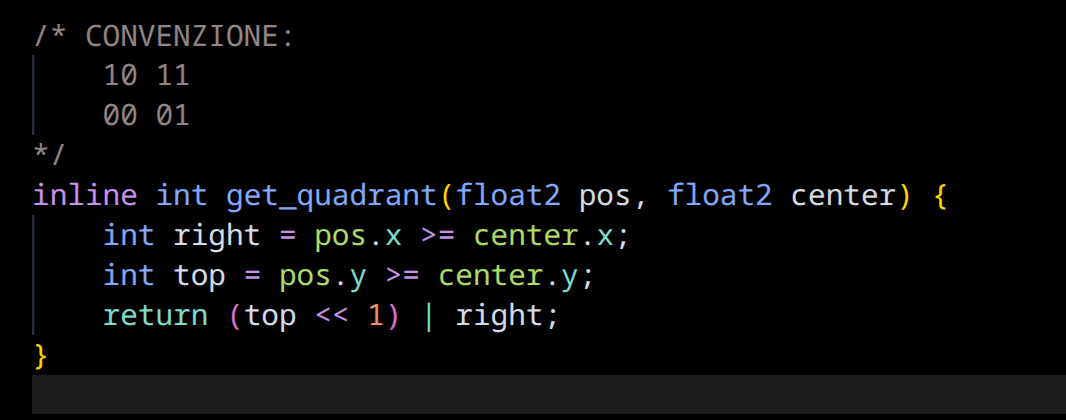
\includegraphics[width=0.75\linewidth]{../images/codequadrant}
		\caption{Convenzione usata nel codice per Barnes-Hut per associare un corpo ad un quadrante nota la posizione del corpo e il centro del quadrante.}
	\end{figure}

Inoltre, l'array \verb|cell_children| contiene al suo interno riferimenti a entità di tipi differenti, ossia nodi e corpi. Stabiliamo la convenzione per cui tutti gli indici che fanno riferimento a nodi dell'albero, hanno indice maggiore o uguale al numero di corpi. Questo significa che, quando memorizziamo l'indice ad un nodo, alla sua posizione del quad-tree va sommato il numero di corpi. Quando invece vogliamo usare l'indice per accedere ad un altro nodo, dobbiamo prima sottrarre la stessa quantità.
	
	In letteratura non si trovano esempi di algoritmi di costruzione di quad-tree paralleli su GPU senza ausilio delle funzioni atomiche: usiamo quindi un approccio seriale, mantenendo tuttavia i dati su GPU, per risparmiare sullo scambio dati CPU-GPU. 
	Ci rifaremo alla costruzione del quad-tree dell'algoritmo originale. Diamo inoltre un limite massimo in altezza all'albero, definito dalla costante \verb|MAX_TREE_DEPTH|, di default posta a 32\footnote{cosa succede quando questo valore viene superato? Andrebbe in realtà implementato un codice di errore da dare alla fine della procedura, per fare capire al codice host che la costruzione del quad-tree non è andata a buon fine, come in \url{https://github.com/bneukom/gpu-nbody}.}.
%\begin{figure}[htpb]
%	\centering
%	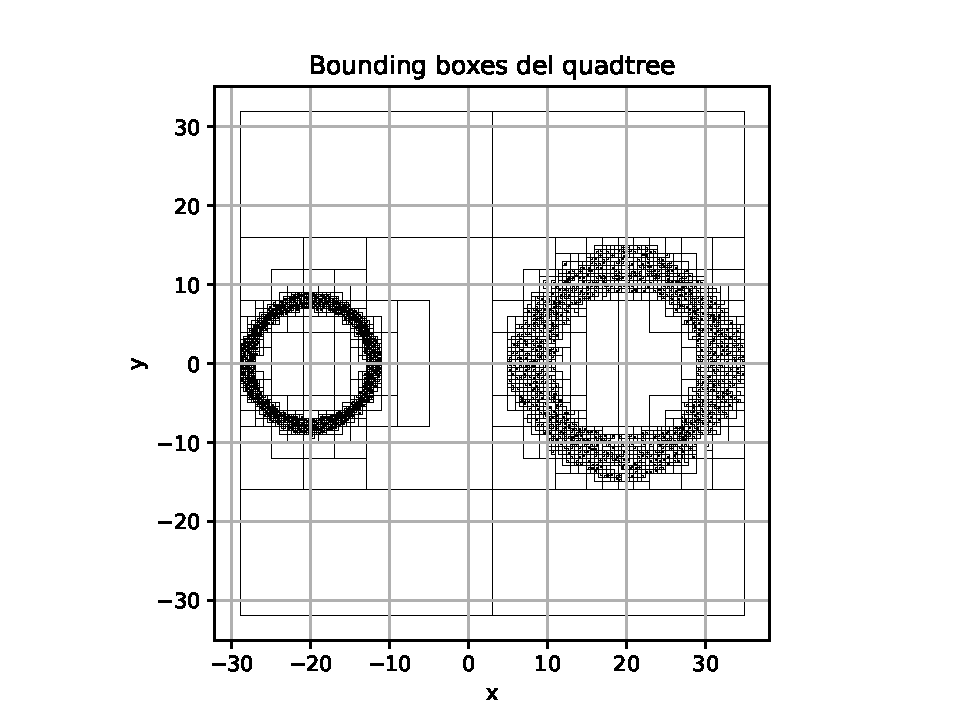
\includegraphics[width=1\linewidth]{../images/bounding-box1}
%\end{figure}
\paragraph{Reset e inizializzazione dell'albero} Questo kernel si occupa del reset della struttura ad albero. Vengono posti nulli i valori del centro di ciascun nodo e dell'halfsize, a -1 le masse e gli indici dei figli. Il kernel con $id=0$ fa uno step in più, ossia settare la posizione del centro e l'halfsize in funzione del risultato della riduzione. Questo kernel in realtà viene eseguito prima della costruzione del quad-tree, ma ai fini della spiegazione, abbiamo preferito introdurlo dopo. Viene lanciato per ciascun nodo dell'albero.

\paragraph{Propagazione delle masse e dei centri di massa}
In letteratura gli approcci ottimali per la summarize-tree sfruttano spesso funzioni atomiche, che non sono state oggetto dei nostri studi; tuttavia, è possibile implementare un kernel da lanciare più volte per compiere lo stesso lavoro.

Il kernel funziona in questo modo: dato un nodo $A$, calcolane la massa (e il centro di massa) osservandone i figli. Se uno di questi figli ha valori non inizializzati (questo avviene quando non si è ancora calcolata la loro massa), esci dal kernel e non modificare la massa del nodo (e nemmeno il centro di massa). 
Questo kernel va lanciato sull'intero quad-tree per un numero di volte pari alla sua altezza, ottenendo una sorta di ``onda'' di pesi che si propagano dal basso verso l'alto. Useremo un ciclo for nel codice host che itera per \verb|MAX_TREE_DEPTH| volte. Il rischio è che l'algoritmo lanci kernel a vuoto quando si è già raggiunta l'altezza \verb|MAX_TREE_DEPTH|. Andrebbe inoltre integrato un modo per evitare passaggi ripetuti quando la massa è già stata calcolata.

\begin{algorithm}[h]
	\caption{Summarize tree (propagazione masse e centri di massa)}
	\begin{algorithmic}[1]
		\Require array del quad-tree $QT$, array dei corpi $C$
		\State $i \gets$ id globale del work-item
		\If{$i >= \operatorname{len}(QT)$}
		\Return
		\EndIf
		\State $\textit{total-mass}\gets 0$
		\State $\textit{center-of-mass}\gets (0,\,0)$
		\State $\textit{weighted-pos}\gets (0,\,0)$
		\ForAll {figli di $QTree[i]$}
		\State $j \gets \text{indice del figlio}$
		\If {$j$ è un indice valido}
		\State $\textit{total-mass} \gets \textit{total-mass} + QT[j]_{mass}$
		\State $\textit{weighted-pos} \gets QT[j]_{pos} \cdot QT[j]_{mass}$
		\Else
		\State\Return
		\EndIf
		\EndFor
		\State $QT[i]_{mass} \gets \textit{total-mass}$
		\State $QT[i]_{\textit{center-of-mass}} \gets \textit{weighted-pos} / \textit{total-mass}$
	\end{algorithmic}
\end{algorithm}

In realtà, nelle istruzioni 9-15 va considerato pure un controllo sul tipo di figlio. $j$ potrebbe infatti essere un indice ad un nodo o un indice ad un corpo. Nel primo caso il calcolo coinvolgerà l'accesso ad un altro slot del quad-tree, nel secondo caso ad uno slot dell'array dei corpi $C$.
	
\paragraph{Calcolo dell'accelerazione usando il quad-tree}
Questa parte dell'algoritmo è imbarazzantemente parallelizzabile: tuttavia, l'algoritmo di attraversamento di un albero come il quad-tree, se non implementabile tramite ricorsione, richiede l'utilizzo di uno stack, il che rende questo kernel un altro elemento  di studio interessante.
Il kernel va lanciato su ciascuno dei corpi (chiameremo il nostro corpo $C[i]$), e procede nel seguente modo:
\begin{enumerate}
	\item si inserisce nello stack la radice del quad-tree (ossia l'intero sistema);
	\item finché lo stack non è vuoto, si estrae un elemento dallo stack;
	\item se l'elemento è un corpo, calcola regolarmente l'accelerazione indotta da quest'ultimo su $C[i]$. Se il corpo estratto è $C[i]$ stesso, si ignora;
	\item se l'elemento è un nodo associato a una cella che \textbf{non} contiene $C[i]$, possiamo verificare la condizione
	\begin{equation}
	\dfrac{\text{dimensione della cella}}{\text{distanza dal centro di massa della cella}} < \theta,
	\end{equation}
	se questa è vera, allora possiamo calcolare l'accelerazione sull'intero albero che ha come radice il nodo in questione usando la sua massa e il uso centro di massa come posizione;
	\item  se nessuna tra le condizioni in 3 e 4 sono rispettate, allora si inseriscono i quattro figli del nodo nello stack;
\end{enumerate}
La condizione relativa al coefficiente $\theta$ può essere riformulata in modi equivalenti, che permettono di risparmiare su operazioni di radici quadrate e divisioni. Nel nostro caso, useremo
\begin{equation}
	(\text{dimensione della cella})^2 < (\text{distanza dal centro di massa della cella})^2 \cdot \theta^2.
\end{equation} 


\paragraph{Aggiornamento di velocità e posizione}
Questi ultimi due kernel sono uguali a quelli del metodo naive, quindi non verranno approfonditi ulteriormente.

\subsection{L'algoritmo complessivo}
\begin{algorithm}[htp]
	\caption{Simulazione $n$-body Barnes-Hut}
	\begin{algorithmic}[1]
		\Require array dei corpi $C$, $n = |C|$, delta tempo $dt$, numero di  iterazioni $t$
		\For {$\log_2n$}
		\State lancia kernel \textbf{riduzione minimo} per ogni corpo rimanente
		\EndFor
		\For {$\log_2n$}
	\State lancia kernel \textbf{riduzione massimo} per ogni corpo rimanente
	\EndFor
	\State lancia $n$ kernel di \textbf{reset e inizializzazione dell'albero}, uno per ogni corpo
	\State lancia 1 kernel di \textbf{costruzione seriale dell'albero}
	\For{MAX TREE DEPTH}
	\State lancia kernel \textbf{propagazione masse e centri di massa} per ogni possibile cella del quad-tree
	\EndFor
	\State lancia $n$ kernel \textbf{calcolo dell'accelerazione}, uno per ogni corpo 
	\State lancia $n$ kernel \textbf{calcolo della velocità} per $dt/2$, uno per ogni corpo \Comment{Mezzo passo di leapfrog}
	\For{$t$}
	\State lancia $n$ kernel \textbf{calcolo della posizione}, uno per ogni corpo 
	\For {$\log_2n$}
	\State lancia kernel \textbf{riduzione minimo} per ogni corpo rimanente
	\EndFor
	\For {$\log_2n$}
	\State lancia kernel \textbf{riduzione massimo} per ogni corpo rimanente
	\EndFor
	\State lancia $n$ kernel di \textbf{reset e inizializzazione dell'albero}, uno per ogni corpo
	\State lancia 1 kernel di \textbf{costruzione seriale dell'albero}
	\For{MAX TREE DEPTH}
	\State lancia kernel \textbf{propagazione masse e centri di massa} per ogni possibile cella del quad-tree
	\EndFor
	\State lancia $n$ kernel \textbf{calcolo dell'accelerazione}, uno per ogni corpo 
	\State lancia $n$ kernel \textbf{calcolo della velocità} per $dt/2$, uno per ogni corpo 
	\EndFor
	\end{algorithmic}
\end{algorithm}

\newpage
\subsection{Benchmarking}
La nostra implementazione dell'algoritmo Barnes-Hut si compone di molteplici kernel:
\begin{enumerate}
	\item riduzione per trovare il minimo;
	\item riduzione per trovare il massimo;
	\item reset dell'albero;
	\item costruzione dell'albero;
	\item propagazione delle masse e dei centri di massa nell'albero;
	\item calcolo dell'accelerazione;
	\item aggiornamento della velocità;
	\item aggiornamento della posizione.
\end{enumerate}

Tra questi passaggi, 1, 2, 3, 7 e 8 risultano essere quelli meno onerosi della nostra implementazione. Fissiamo $\theta = 0.1$ e scegliamo come GPU di riferimento la AMD RX6600. In figura~\ref{fig:bhkernelcomparisontheta01}, il kernel più oneroso appare essere quello di reset dell'albero, il che risulta riconducibile all'alto numero di accessi in memoria richiesti.

\begin{figure}[tph]
	\centering
	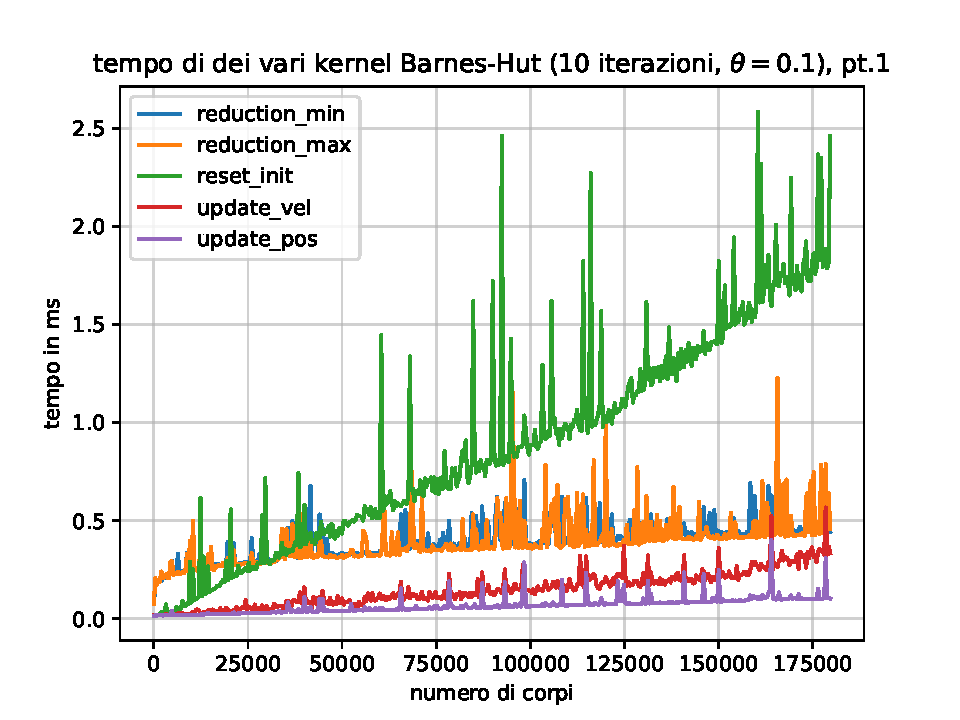
\includegraphics[width=0.7\linewidth]{../images/bh_kernel_comparison_theta0_1}
	\label{fig:bhkernelcomparisontheta01}
	\caption{Tempo dei kernel di Barnes-Hut per la riduzione (minimo e massimo della bounding-box), reset e inizializzazione dell'albero, aggiornamento della velocità e della posizione.}
\end{figure}

I passaggi 4, 5 e 6 sono invece molto più onerosi dei precedenti. In particolare, nella nostra implementazione, la costruzione dell'albero (4) seriale è un vero e proprio collo di bottiglia per il resto dell'algoritmo. La propagazione delle masse (5) non cresce in maniera significativa ($\sim273ms$ su $\sim 180000$ particelle), ma più velocemente dei kernel precedenti. Citiamo per ultimo il kernel dedicato al calcolo dell'accelerazione (6): l'intero algoritmo Barnes-Hut punta sull'ottimizzazione di questo passaggio tramite l'approssimazione sensibile al parametro $\theta$. Ne consegue che l'algoritmo vada valutato anche in funzione di quest'ultimo. Se in figura~\ref{fig:bhkernelcomparisontheta01pt2} abbiamo i kernel 4,5 e 6 con $\theta = 0.1$, gli stessi sono messi a confronto con $\theta = 0.5$ in figura~\ref{fig:bhkernelcomparisontheta05pt2}. Osserviamo un importante guadagno in prestazioni, che sottolinea la potenza dell'approssimazione Barnes-Hut.

\begin{figure}[tph]
	\centering
	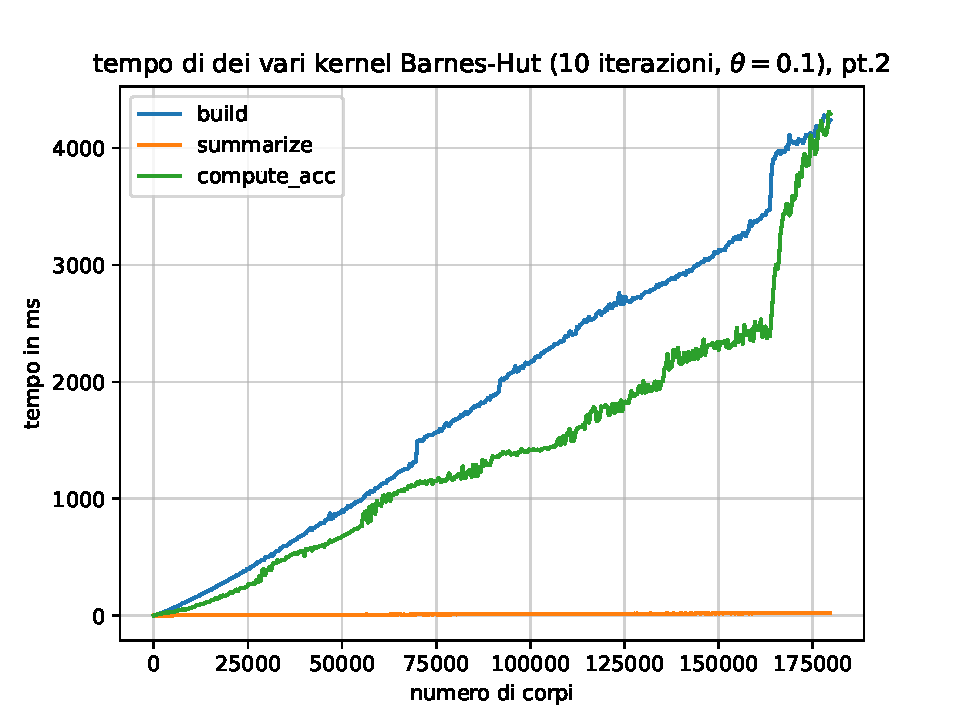
\includegraphics[width=0.6\linewidth]{../images/bh_kernel_comparison_theta0_1pt2}
	\caption{Plot dei tempi dei kernel di costruzione (seriale) dell'albero, propagazione di masse e centri di massa e calcolo dell'accelerazione in funzione del numero di corpi, con $\theta = 0.1$}
	\label{fig:bhkernelcomparisontheta01pt2}
\end{figure}

\begin{figure}[tph]
	\centering
	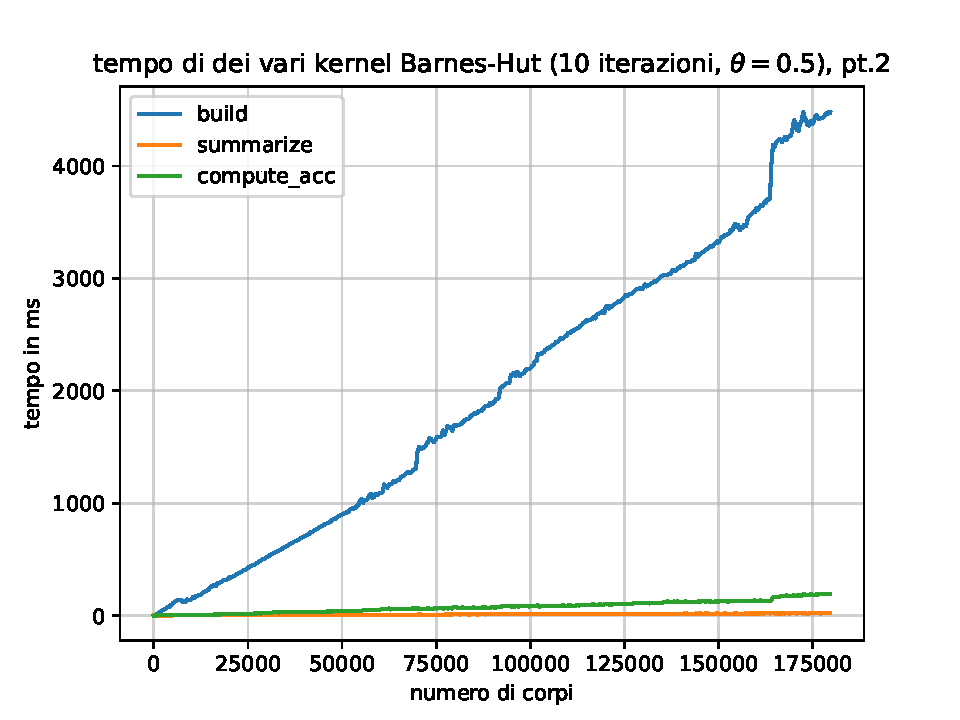
\includegraphics[width=0.6\linewidth]{../images/bh_kernel_comparison_theta0_5pt2}
	
	\caption{Plot dei tempi dei kernel di costruzione (seriale) dell'albero, propagazione di masse e centri di massa e calcolo dell'accelerazione in funzione del numero di corpi, con $\theta = 0.1$}
	\label{fig:bhkernelcomparisontheta05pt2}
\end{figure}

Va tuttavia specificata una cosa quando desideriamo mettere a confronto l'approccio naive a quello Barnes-Hut: il vantaggio asintotico diventa un vantaggio effettivo solo con un numero di particelle molto alto. A causa delle risorse ridotte a nostra disposizione (e al bottleneck del build-tree seriale), non ci sarà possibile allocare abbastanza particelle per assistere al vantaggio di BH. Tuttavia, decidendo di ignorare il tempo degli altri kernel, possiamo mettere a confronto esclusivamente i tempi di calcolo delle accelerazioni nei rispettivi algoritmi. Dalla figura~\ref{fig:bhvsnaiveacc} emerge come la scelta del valore di $\theta$ sia cruciale per ottenere lo speedup promesso dall'algoritmo, molto più della scelta dell'hardware: per $\theta = 0.1$ il calcolo dell'accelerazione è più lento che nella simulazione naive. Per $\theta = 0.5$, cresce in maniera simile alla summarize tree.s
\begin{figure}[tbph]
	\centering
	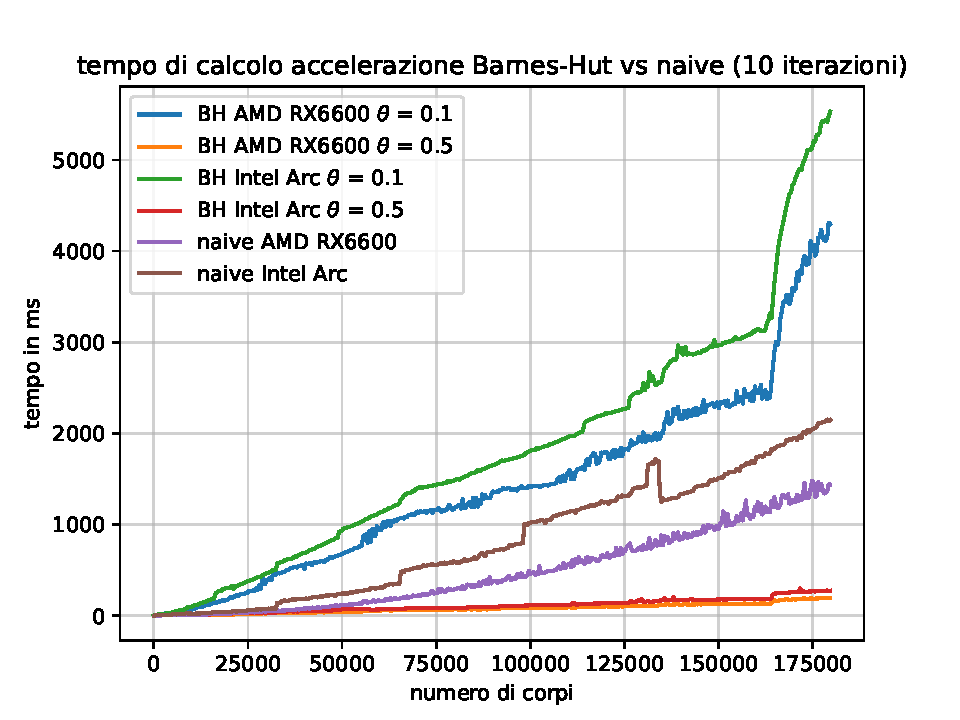
\includegraphics[width=0.6\linewidth]{../images/bh_vs_naive_acc}
	\caption{Plot dei tempi dei kernel di calcolo dell'accelerazione nell'approccio naive e nell'approccio Barnes-Hut con $\theta = 0.1$ e $\theta = 0.5$.}
	\label{fig:bhvsnaiveacc}
\end{figure}


%{\huge TODO inserire il confronto per theta = 0.1, 0.2, 0.3, 0.4, 0.5, 0.6, 0.7, 0.8}

\section{Simulazione Barnes-Hut ibrida}
La costruzione seriale del quad-tree rappresenta la principale fonte di overhead nella nostra attuale implementazione dell'algoritmo Barnes-Hut totalmente su GPU. L'obiettivo era quello di ridurre al minimo i costi di trasferimento della memoria da CPU a GPU e viceversa, usando esclusivamente un kernel eseguito da un solo work-item per la costruzione del quad-tree. 
Tuttavia, usare un work-item della GPU rispetto che la CPU, rappresenta un enorme collo di bottiglia a causa della frequenza di clock più bassa. Sfruttiamo il meglio dei due hardware, GPU e CPU, affidando proprio alla seconda la costruzione dell'albero, ossia l'unico task affrontato in maniera esclusivamente seriale. 

\subsection{Benchmarking}
Con questa implementazione ibrida dell'algoritmo Barnes-Hut, riusciamo finalmente a ottenere un vantaggio sull'approccio naive visibile col numero attuale di particelle coinvolte. In figura~\ref{fig:naivebhtotalms} mettiamo a confronto
\begin{itemize}
	\item Algoritmo naive su Intel Arc;
	\item Algoritmo naive su AMD RX6600;
	\item Algoritmo naive su AMD Raphael;
	\item Algoritmo Barnes-Hut puro su GPU, Intel Arc, $\theta = 0.5$;
	\item Algoritmo Barnes-Hut puro su GPU, AMD RX6600, $\theta = 0.5$;
	\item Algoritmo Barnes-Hut ibrido CPU-GPU, Intel Arc, $\theta = 0.5$;
	\item Algoritmo Barnes-Hut ibrido CPU-GPU, AMD RX6600, $\theta = 0.5$.
\end{itemize} 

\begin{figure}[tph]
	\centering
	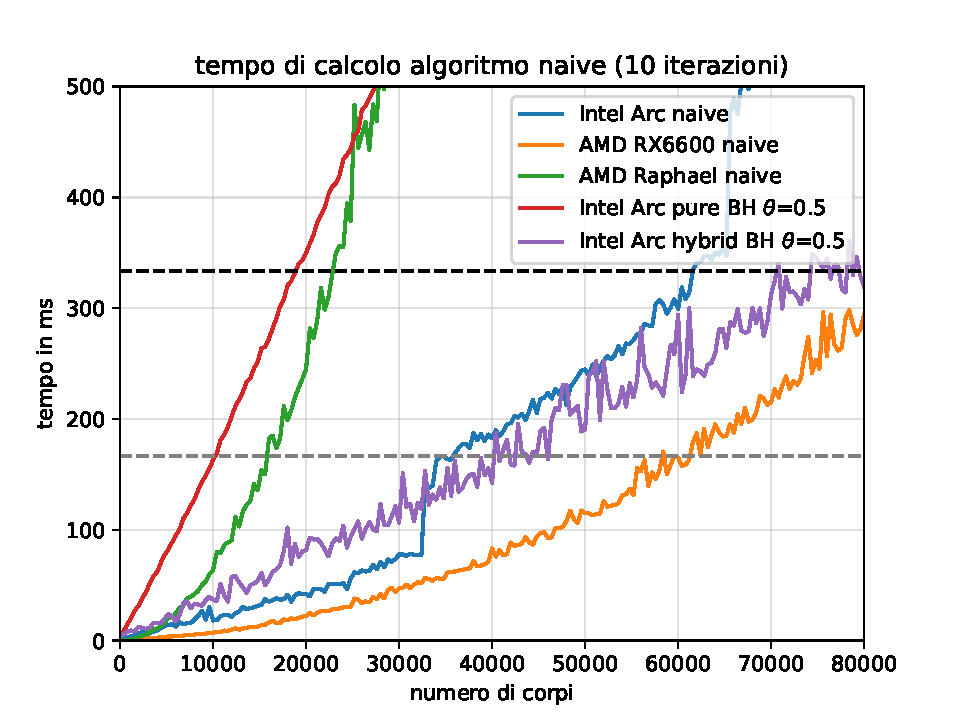
\includegraphics[width=0.8\linewidth]{../images/naive_bh_total_ms}
	\caption{Confronto tra algoritmo naive su Intel Arc, AMD RX6600 e AMD Raphael,
		algoritmo Barnes-Hut puro GPU su Intel Arc e AMD RX6600 con $\theta = 0.5$,
		algoritmo Barnes-Hut ibrido CPU-GPU su Intel Arc e AMD RX6600 con $\theta = 0.5$.}
	\label{fig:naivebhtotalms}
\end{figure}
%ù
I risultati ottenuti ci portano a una conclusione: la frequenza della CPU domina sul passaggio seriale, rendendo vano il risparmio sulle operazioni di lettura e scritta da GPU a CPU e viceversa.
Questo approccio ibrido rende la nostra implementazione su Barnes-Hut viabile per applicazioni real-time. In particolare, questo vantaggio si ottiene a numeri molto più bassi di particelle sulla Intel Arc rispetto all'AMD RX6600, il che è riconducibile a due motivi fondamentali: un processore più performante, e l'uso della mappatura in memoria (molto conveniente sulle GPU integrate).

	
\section{Ricerca di minimo e del massimo con sliding window}
L'ultima parte della nostra relazione, approfondirà un'ottimizzazione sulla prima parte dell'algoritmo, ossia la ricerca del minimo e del massimo per la definizione della bounding box. 
Seppur nelle implementazioni fornite fino ad ora abbiamo usato un approccio alle riduzioni parallele basato su un albero dei confronti, esistono approcci migliori che permettono di
	\begin{enumerate}
		\item ridurre il numero di lanci dei kernel da $2\log_2n$ a 2;
		\item ridurre il numero di accessi alla memoria globale, sfruttando quanto possibile la local memory.
	\end{enumerate}
	L'approccio che permette di ottenere questi risultati, è chiamato sliding window (con local memory). Inoltre, andremo ad unificare la ricerca del minimo e del massimo in una sola ricerca, in modo da ridurre il numero di accessi in memoria.
	
	\subsection{I kernel}
	Per questo approccio alla riduzione, usiamo esclusivamente due kernel, lanciati una volta a testa. Nel codice host, questi si integreranno al posto dei due cicli dedicati alle riduzioni. Inoltre, la dimensione dei buffer dedicati alle riduzioni, potrà essere ridotta a un \verb|sizeof(cl_float2) * nwg|.
	
	\paragraph{Riduzione con sliding window, kernel primo} 
	Ciascun work-item esegue il seguente codice:
	\begin{enumerate}
		\item impostare minimo e massimo a $-\infty$  e $+\infty$ (variabili private di ogni work-item);
		\item si tratta il vettore a due componenti delle posizioni, come un vettore a 16 componenti;
		\item fino alla fine delle ``sedicine'', si fa una riduzione vettorizzata per trovare minimo e massimo. Alla fine di ogni ciclo, il work-item fa un salto pari alla dimensione della global size\footnote{questo pattern affrontato a lezione si chiama stride, e migliore la coelescenza della memoria.}, che è uguale al prodotto tra numero di work item e local work size;
		\item ogni work item fornisce il proprio minimo e massimo privato in due array in local memory;
		\item si effettua una riduzione parallela in local memory;
		\item il primo work-item di ciascun work group deposita i propri risultati in due array a parte.
	\end{enumerate}
	
	Questo kernel viene lanciato su un numero di kernel pari al prodotto tra la local work size e il numero di work group.
	
	\paragraph{Riduzione con sliding window, kernel secondo} 
	\begin{enumerate}
	\item impostare minimo e massimo a $-\infty$  e $+\infty$ (variabili private di ogni work-item);
	\item fino alla fine delle entries, i work item effettuano riduzioni parallele per trovare minimo e massimo, facendo salti analoghi ai precedenti (stride);
	\item il minimo e il massimo di ciascun work-item viene scritto in local memory;
	\item ultima riduzione parallela in local memory, analoga a quella del primo kernel;
	\item il primo work-item dell'unico work group operante, scrive il risultato definitivo della ricerca del minimo e del massimo sul buffer dedicato.
	\end{enumerate}
	Questo kernel, come già accennato sull'ultimo passaggio, è lanciato su un singolo work-group, in quanto la global work size è pari alla local work size.
	
	\subsection{I confronti vettorizzati}
	L'ultima cosa che vale la pena approfondire è il pattern dei confronti usato per la riduzione parallela con istruzioni SIMD (riduzione vettorizzata).
	Se negli esempi affrontati a lezione, si è sempre optato per confrontare le componenti di indice pari a quelle di indice dispari, nel nostro contesto, dopo aver castato il puntatore a \verb|global float2| in un puntatore a \verb|global float16|, è stato necessario adottare l'uso dei suffissi \verb|.lo| e \verb|.hi|. Di seguito, la motivazione:
	
	\begin{verbatim}
	supponiamo che le componenti siano in ordine decrescente
	         
	schema di riduzione vettorizzata con .lo e .hi
	
	x0 y0 x1 y1 x2 y2 x3 y3 x4 y4 x5 y5 x6 y6 x7 y7
	
	x0 y0 x1 y1 x2 y2 x3 y3 
	|| || || || || || || ||
	x4 y4 x5 y5 x6 y6 x7 y7
	
	x0 y0 x1 y1 x2 y2 x3 y3 
	|| || || || || || || ||
	x4 y4 x5 y5 x6 y6 x7 y7
	
	x0 y0 x1 y1
	|| || || ||
	x2 y2 x3 y3 
	
	x0 y0 
	|| ||
	x1 y1
	
	
	schema di riduzione vettorizzata con .even e .odd
	
	x0 y0 x1 y1 x2 y2 x3 y3 x4 y4 x5 y5 x6 y6 x7 y7
	
	x0 x1 x2 x3 x4 x5 x6 x7
	|| || || || || || || ||    confronto anomalo!!
	y0 y1 y2 y3 y4 y5 y6 y7
	\end{verbatim} 
	
	In altre parole, desideriamo confrontare le componenti orizzontali solo con altre componenti orizzontali, e analogamente con le componenti verticali. 
	
	\paragraph{Una nota importante} Il casting necessario per il confronto vettorizzato, necessità però una garanzia: il numero di corpi deve essere un multiplo di 8 in quanto, avendo i corpi due componenti, garantisce che il casting sia sicuro. Per evitare di dover gestire casi limite, integriamo semplicemente un controllo sul numero dei corpi prima dell'intera simulazione.
	

	\subsection{Ricerca dei migliori valori di local work size e work group}
	Proprio a causa dell'uso della local memory, sarà necessario comprendere come assegnare i valori di local work size, e il numero di work group per compute unit. La ricerca attuale sarà svolta per la GPU AMD RX6600. Cambiando hardware, i risultati possono variare. Testeremo per local work size $\in \{64, 128, 256\}$, e numero di work group per compute unit $\in \{1, 2, 4, 8, 16\}$. Tutte queste combinazioni, saranno valutate su varie quantità di corpi.
	I primi risultati che forniamo, sono quelli di 50 iterazioni su 180 000 particelle, in tabella~\ref{tab:1}, ai quali affianchiamo quelli di 50 iterazioni su 90 000 particelle della tabella~\ref{tab:2}.
	
	I dati raccolti non sono molti, e andrebbe fatto uno studio più estensivo. Tuttavia, possiamo fare alcune osservazioni:
	\begin{itemize}
		\item il tempo di $k1$ domina sempre il tempo di $k2$;
		\item la dimensione del problema rende più o meno rilevante la scelta dei parametri;
		\item avere pochi work-item aumenta il numero di operazioni svolte in maniera sequenziale, ma troppi work-group aumentano il numero di riduzioni da effettuare in $k2$.
	\end{itemize}
	\begin{table}[h]
		\centering
		\begin{tabular}{c|c|c|c|c}
		$k1$ & $k2$ & $k1 + k2$ & $lws$ & $mwg/cu$\\
		\hline
		0.918175 & 0.188681 & 1.106856 &  \textbf{64} &  \textbf{1} \\
		0.843773 & 0.181842 & 1.025615 &  64 &  2 \\
		0.503931 & 0.143165 & 0.647096 &  \textbf{64} &  \textbf{4} \\
		0.534926 & 0.171360 & 0.706286 &  64 &  8 \\
		0.537650 & 0.259646 & 0.797296 &  64 & 16 \\
		0.825895 & 0.197242 & 1.023137 & 128 &  1 \\
		0.693293 & 0.197322 & 0.890615 & 128 &  2 \\
		0.516247 & 0.159002 & 0.675249 & 128 &  4 \\
		0.563928 & 0.202364 & 0.766292 & 128 &  8 \\
		0.678490 & 0.235441 & 0.913931 & 128 & 16 \\
		0.729054 & 0.202366 & 0.931420 & 256 &  1 \\
		0.677050 & 0.204363 & 0.881413 & 256 &  2 \\
		0.684891 & 0.203842 & 0.888733 & 256 &  4 \\
		0.724611 & 0.222083 & 0.946694 & 256 &  8 \\
		0.642088 & 0.238005 & 0.880093 & 256 & 16 \\
		\end{tabular}
		\label{tab:1}
		\caption{Tempi dei kernel di riduzione con sliding window, per $n = 180000$, su 50 iterazioni}
	\end{table}
	
		\begin{table}[h]
		\centering
		\begin{tabular}{c|c|c|c|c}
			$k1$ & $k2$ & $k1 + k2$ & $lws$ & $mwg/cu$\\
			\hline
			0.292004 &0.126880 &0.418884 &\textbf{64} &\textbf{1}\\
			0.248483 &0.120403 &0.368886 &64 &2\\
			0.249324 &0.129363 &0.378687 &64 &4\\
			0.248928 &0.149003 &0.397931 &64 &8\\
			0.232481 &0.168882 &0.401363 &64 &16\\
			0.247884 &0.125444 &0.373328 &128 &1\\
			0.251406 &0.134002 &0.385408 &128 &2\\
			0.237562 &0.119363 &0.356925 &\textbf{128} &\textbf{4}\\
			0.240686 &0.135482 &0.376168 &128 &8\\
			0.245044 &0.157081 &0.402125 &128 &16\\
			0.255086 &0.139725 &0.394811 &256 &1\\
			0.249884 &0.126400 &0.376284 &256 &2\\
			0.238763 &0.124524 &0.363287 &256 &4\\
			0.232525 &0.123122 &0.355647 &256 &8\\
			0.280804 &0.115242 &0.396046 &256 &16\\
			
		\end{tabular}
		\label{tab:2}
		\caption{Tempi dei kernel di riduzione con sliding window, per $n = 90000$, su 50 iterazioni}
	\end{table}
	
	\newpage
	\subsection{Confronto: riduzione parallela naive e sliding window}
	Questo approccio permette di ottenere un vantaggio non indifferente su quanto ottenuto con le riduzioni parallele naive delle precedenti soluzioni. Il numero di lanci dei kernel fisso a 2 piuttosto che $\log_2 n$, le operazioni vettorizzate SIMD e l'uso della local memory, con un'opportuna scelta dei parametri rispetto all'hardware e alla dimensione della simulazione, permette di abbassare radicalmente le tempistiche per l'ottenimento della dimensione della bounding box. Concludiamo questo report con un confronto tra le tempistiche della ricerca unificata. Fisseremo $lws=64$ e $nwg/cu = 4$.
	\newpage
	
	\begin{table}[h]
		\centering
		\begin{tabular}{c|c|c}
			tempo di $kmin + kmax$ in ms & tempo di $k1+k2$ in ms & $\textit{body count}$\\
			\hline
			0.420529 & 0.056282 &   4000 \\
			0.476329 & 0.049640 &   8000 \\
			0.521727 & 0.058682 &  12000 \\
			0.516364 & 0.063281 &  16000 \\
			0.586213 & 0.056000 &  20000 \\
			0.547727 & 0.060882 &  24000 \\
			0.562649 & 0.058843 &  28000 \\
			0.58813 & 0.072202 &  32000 \\
			0.666406 & 0.066161 &  36000 \\
			0.605535 & 0.071081 &  40000 \\
			0.582808 & 0.081240 &  44000 \\
			0.600969 & 0.095842 &  48000 \\
			0.623049 & 0.081882 &  52000 \\
			0.651688 & 0.086120 &  56000 \\
			0.673891 & 0.082040 &  60000 \\
			0.670965 & 0.088523 &  64000 \\
			0.665493 & 0.080882 &  68000 \\
			0.702813 & 0.081922 &  72000 \\
			0.692888 & 0.171443 &  76000 \\
			0.727525 & 0.113520 &  80000 \\
			0.775973 & 0.089761 &  84000 \\
			0.826889 & 0.102041 &  88000 \\
			0.808377 & 0.091680 &  92000 \\
			0.816087 & 0.100282 &  96000 \\
			0.854855 & 0.106202 & 100000 \\
			0.816576 & 0.139723 & 104000 \\
			0.844415 & 0.148284 & 108000 \\
			0.949291 & 0.142283 & 112000 \\
			0.938171 & 0.148723 & 116000 \\
			0.9593 & 0.160402 & 120000 \\
			1.029618 & 0.167161 & 124000 \\
			1.002053 & 0.202563 & 128000 \\
			1.070942 & 0.188643 & 132000 \\
			1.081577 & 0.184522 & 136000 \\
			1.062177 & 0.191801 & 140000 \\
			1.16534 & 0.206162 & 144000 \\
			1.120819 & 0.161443 & 148000 \\
			1.220338 & 0.188121 & 152000 \\
			1.161228 & 0.203242 & 156000 \\
			1.128337 & 0.194963 & 160000 \\
			1.222573 & 0.215324 & 164000 \\
			1.196777 & 0.207443 & 168000 \\
			1.27554 & 0.223962 & 172000 \\
			1.253379 & 0.227482 & 176000 \\
		\end{tabular}
		\caption{Tabella dei tempi al variare del numero dei corpi, dei kernel di riduzione parallela naive (albero dei confronti) e dei kernel di riduzione tramite sliding window con global memory}
	\end{table}
	
	Dalla tabella, è evidente il vantaggio ottenuto: la riduzione con sliding window è sempre dalle 8 volte alle 5 volte più veloce dell'approccio con riduzione naive.
	\newpage
	
	\newpage
	\printbibliography
	
\end{document}          
